\chapter[Nodo IoT y Red de Campo]{Nodo IoT y Red de Campo}
\label{chap:nodo-iot}

\section{Introducción}
\label{sec:nodo-intro}

Este capítulo describe el nodo IoT que vincula cada medidor inteligente con la red de campo \emph{mesh}. El análisis sigue el recorrido del dato: desde su origen en el \textbf{medidor trifásico} y su pila de comunicación \textbf{DLMS/COSEM} sobre RS-485, pasando por el \textbf{modelo de dispositivo} LwM2M, la \textbf{implementación del firmware} en Zephyr~RTOS, hasta la transmisión por la \textbf{red Thread} en malla (\emph{mesh}).

§\ref{sec:nodo-hardware} presenta la plataforma de referencia: SoC~ESP32-C6 con radio IEEE~802.15.4 y transceptor RS-485 con aislamiento galvánico. §\ref{sec:nodo-medidor-dlms} especifica el medidor Emsitech~P2000-T, el protocolo DLMS/COSEM y los 27~códigos OBIS implementados. §\ref{sec:nodo-lwm2m} define el Objeto~10242 (\emph{3-Phase Power Meter}) con sus 27~recursos y el perfil LwM2M configurado en ThingsBoard. §\ref{sec:nodo-firmware} detalla el \emph{firmware} Zephyr~RTOS con pila CoAP/OpenThread, ciclo principal y estrategias de optimización de sobrecarga. §\ref{sec:nodo-pila-protocolos} describe la red de campo Thread: capa IEEE~802.15.4, topología, auto-formación y direccionamiento IPv6, \textbf{agotando el tema Thread aquí} según la Regla de Exclusión. §\ref{sec:nodo-pruebas} presenta el análisis de carga y las pruebas de latencia que validan H3 ($<$250\,ms).

Los nodos se alimentan directamente desde el puerto auxiliar 5\,V del medidor (27\,mA promedio), sin restricción energética. El piloto valida la pila completa DLMS/COSEM $\rightarrow$ LwM2M $\rightarrow$ CoAP/Thread con 1~medidor físico Emsitech~P2000-T. Los listados de código fuente están disponibles en el repositorio del proyecto\footnote{\url{https://github.com/jsebgiraldo/ami-lwm2m-node}}.


\section{Arquitectura del nodo IoT}
\label{sec:nodo-hardware}

Esta sección describe los requisitos de \emph{hardware} y la plataforma de referencia seleccionada para el piloto. El \emph{firmware} Zephyr que la ejecuta se presenta en §\ref{sec:nodo-firmware}.

\subsection{Requisitos y Plataforma de Referencia}
\label{sec:nodo-hardware-arquitectura}

El diseño requiere un SoC con: (1)~radio IEEE~802.15.4, (2)~soporte Zephyr RTOS con OpenThread, (3)~interfaz UART para RS-485, y (4)~seguridad por \emph{hardware} (AES, ECDSA). Múltiples plataformas cumplen estos requisitos (ESP32-C6, nRF52840, EFR32MG24, entre otros). Para el piloto de validación se seleccionó \textbf{ESP32-C6} (módulo Seeed Studio XIAO~\cite{seeedstudioXIAOESP32C62024}, 21$\times$17,5\,mm) por: factor de forma compacto, radio 802.15.4 nativa con TX hasta +21\,dBm / RX $-$103\,dBm, arquitectura RISC-V de código abierto (\emph{open-source}), y precio \$3,20/u en volumen.

Para comunicación RS-485 con medidores DLMS/COSEM se utiliza un transceptor MAX485 con aislamiento galvánico 2,5\,kV~\cite{seeedstudioRS485Breakout2024}, terminal 3-pin (A+, B$-$, GND) con resistencia terminación 120\,$\Omega$ seleccionable. Conexión vía cable CAT5e al puerto RJ45 del medidor, alimentación 5\,V desde PoE auxiliar (200\,mA disponibles). Consumo sistema completo: 27\,mA @ 5\,V (véase Capítulo~\ref{chap:resultados}).

\begin{figure}[H]
\centering
\begin{minipage}{0.45\textwidth}
    \centering
    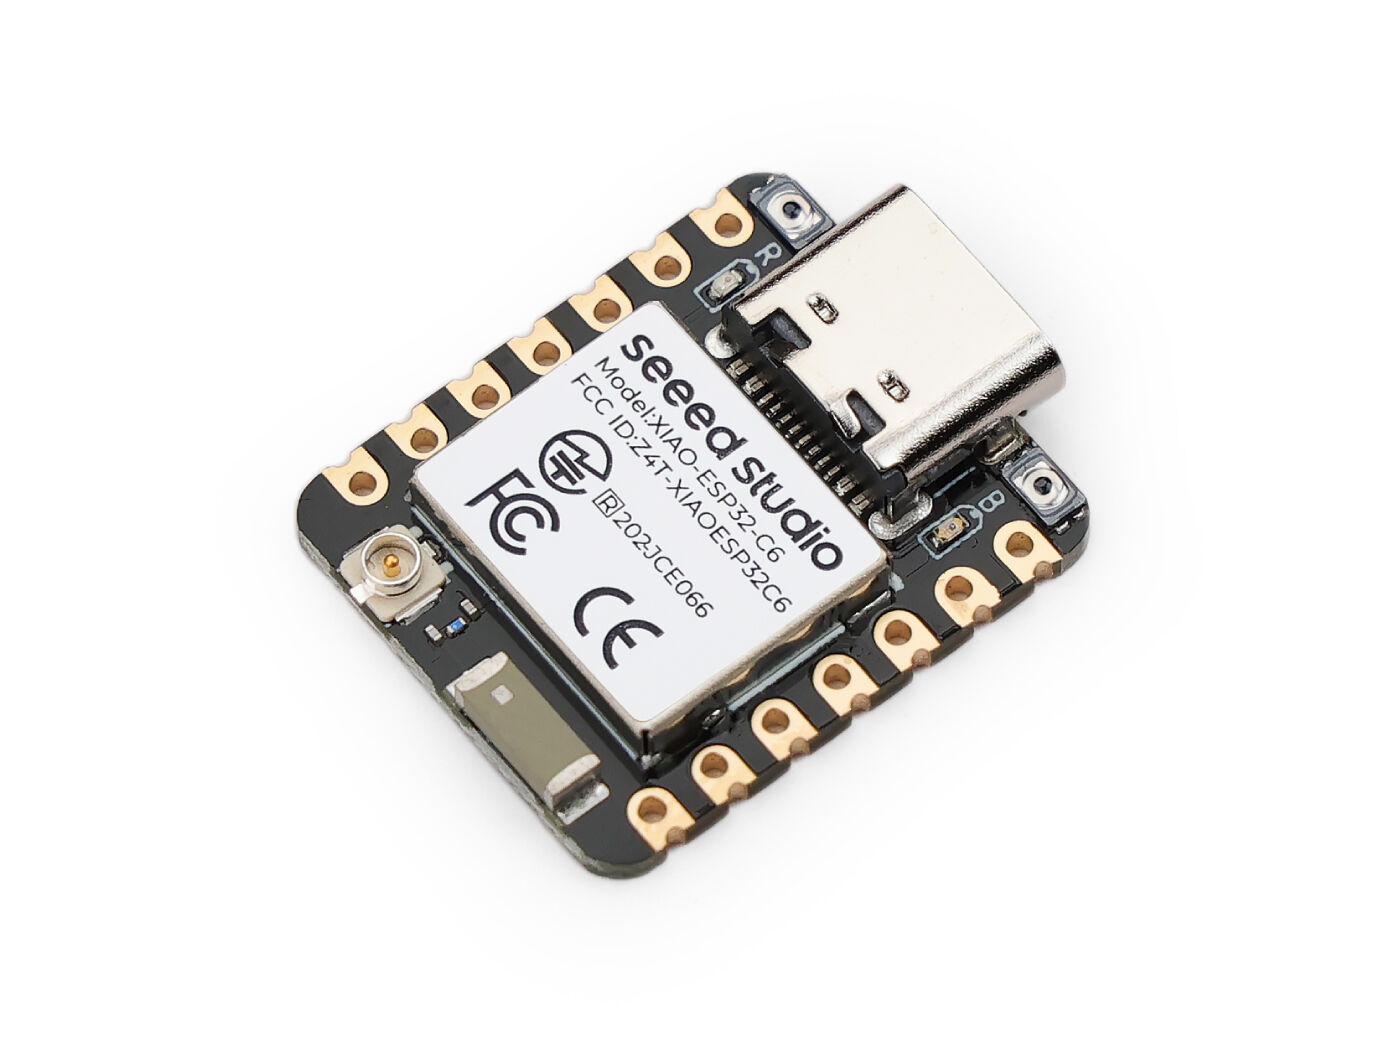
\includegraphics[width=0.9\textwidth]{figures/1-113991254-seeedxiao-esp32c6-45font_1.jpg}
    \small\textbf{(a)} Módulo SoC con radio 802.15.4
\end{minipage}
\hfill
\begin{minipage}{0.45\textwidth}
    \centering
    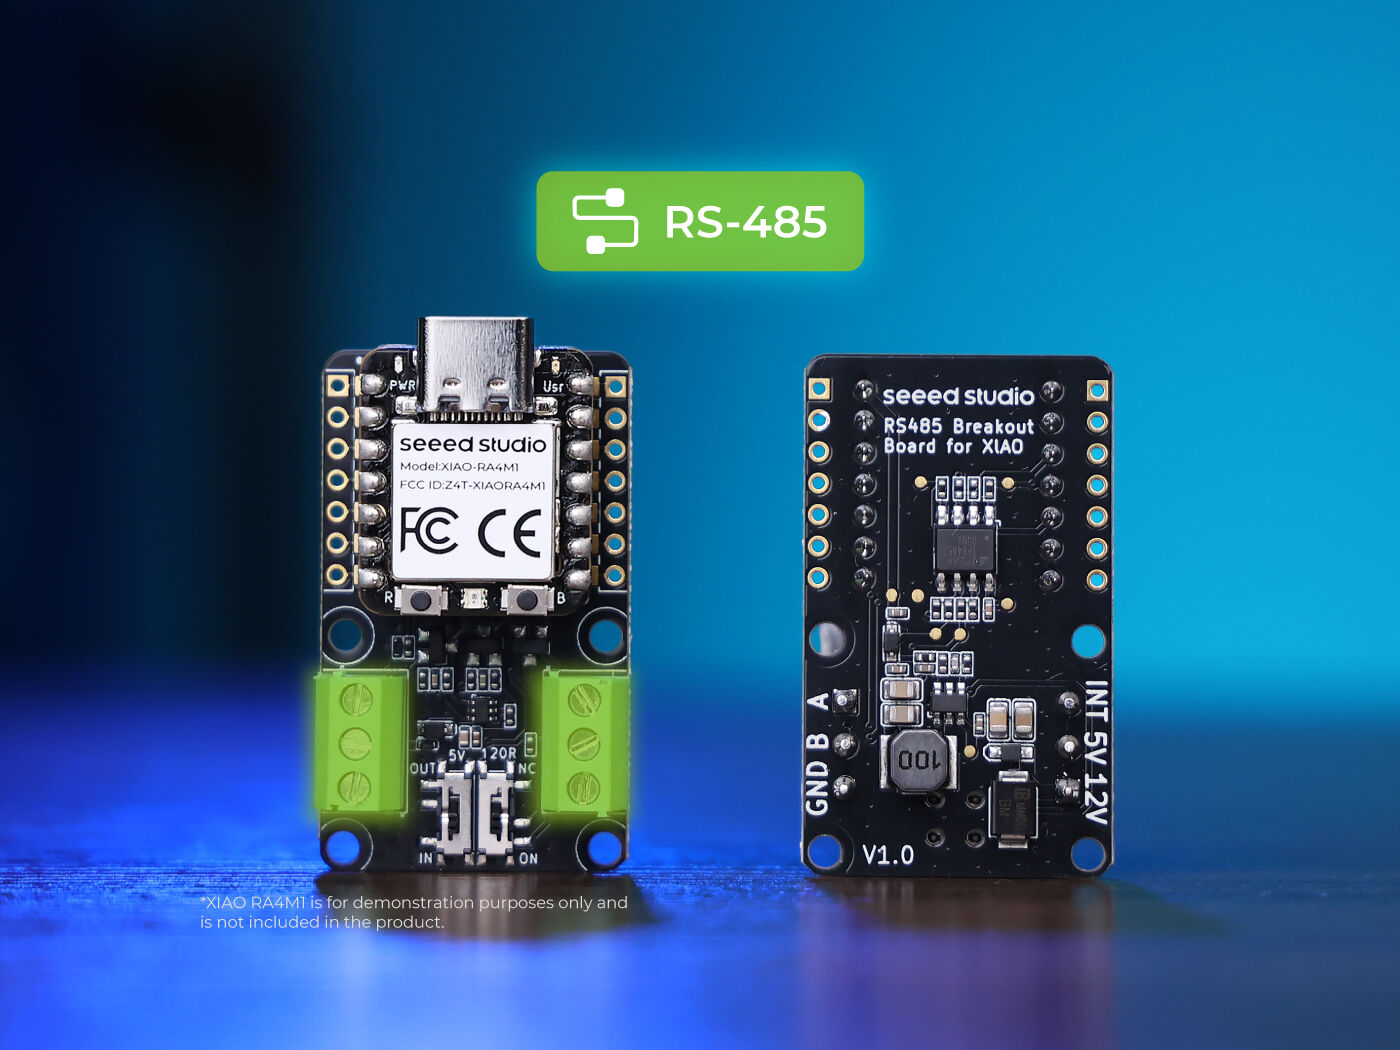
\includegraphics[width=0.9\textwidth]{figures/1-113991354_1.jpg}
    \small\textbf{(b)} Transceptor RS-485 con aislamiento galvánico
\end{minipage}
\caption{Plataforma de referencia utilizada en el piloto. Fuente:~\cite{seeedstudioXIAOESP32C62024,seeedstudioRS485Breakout2024}}
\label{fig:xiao-hardware}
\end{figure}

% Diagrama de bloques TikZ del ESP32-C6 / XIAO ESP32C6 — Nodo IoT Thread
% v3 — Hispanizado, rutas limpias sin cruces, bloques más espaciados

\begin{figure}[ht]
\centering
\resizebox{0.95\textwidth}{!}{%
\begin{tikzpicture}[
  % Estilos base
  blockbase/.style={rounded corners=3pt, minimum height=1.0cm, font=\scriptsize\sffamily,
    inner sep=5pt, line width=0.6pt, align=center},
  block-blue/.style={blockbase, draw=blue!65!black, fill=blue!12,
    drop shadow={shadow xshift=0.4mm, shadow yshift=-0.4mm, opacity=0.15}},
  block-purple/.style={blockbase, draw=purple!65!black, fill=purple!12,
    drop shadow={shadow xshift=0.4mm, shadow yshift=-0.4mm, opacity=0.15}},
  block-green/.style={blockbase, draw=green!50!black, fill=green!10,
    drop shadow={shadow xshift=0.4mm, shadow yshift=-0.4mm, opacity=0.15}},
  block-teal/.style={blockbase, draw=teal!65!black, fill=teal!12,
    drop shadow={shadow xshift=0.4mm, shadow yshift=-0.4mm, opacity=0.15}},
  block-orange/.style={blockbase, draw=orange!65!black, fill=orange!12,
    drop shadow={shadow xshift=0.4mm, shadow yshift=-0.4mm, opacity=0.15}},
  block-red/.style={blockbase, draw=red!60!black, fill=red!10,
    drop shadow={shadow xshift=0.4mm, shadow yshift=-0.4mm, opacity=0.15}},
  soc/.style={draw=blue!70!black, fill=blue!4, rounded corners=5pt,
    line width=1.4pt, inner sep=8pt},
  extblockbase/.style={rounded corners=3pt, minimum height=1.1cm, font=\scriptsize\sffamily,
    inner sep=5pt, line width=0.7pt, align=center,
    drop shadow={shadow xshift=0.3mm, shadow yshift=-0.3mm, opacity=0.12}},
  extblock-green/.style={extblockbase, draw=green!40!black, fill=green!5},
  extblock-purple/.style={extblockbase, draw=purple!55, fill=purple!6},
  extblock-orange/.style={extblockbase, draw=orange!55, fill=orange!6},
  extblock-brown/.style={extblockbase, draw=brown!55, fill=brown!6},
  extblock-red/.style={extblockbase, draw=red!45, fill=red!5},
  extblock-darkred/.style={extblockbase, draw=red!50, fill=red!5},
  extblock-gray/.style={extblockbase, draw=gray!55, fill=gray!6},
  conn/.style={-{Latex[length=2mm]}, line width=0.7pt, #1},
  bidi/.style={{Latex[length=2mm]}-{Latex[length=2mm]}, line width=0.7pt, #1},
]

% === Límite del SoC ===
\draw[soc] (-6.5, -2.8) rectangle (6.5, 4.8);
\node[font=\footnotesize\bfseries\sffamily, blue!70!black] at (0, 4.4) {ESP32-C6 SoC (QFN 5$\times$5\,mm)};

% === CPU ===
\node[block-blue, minimum width=4.0cm, minimum height=1.3cm] (cpu) at (0, 3.2) {};
\node[font=\scriptsize\bfseries\sffamily] at (0, 3.5) {RISC-V RV32IMAC};
\node[font=\scriptsize\sffamily] at (0, 2.95) {Núcleo único @ 160\,MHz (400\,DMIPS)};

% === Memorias ===
\node[block-purple, minimum width=1.8cm] (sram) at (-3.8, 3.2) {SRAM\\512\,KB};
\node[block-purple, minimum width=1.8cm] (rom) at (3.8, 3.2) {ROM\\320\,KB};

% === Radio 802.15.4 ===
\node[block-green, minimum width=3.2cm, minimum height=1.3cm] (radio154) at (-3.0, 1) {};
\node[font=\scriptsize\bfseries\sffamily] at (-3.0, 1.35) {Radio IEEE 802.15.4};
\node[font=\scriptsize\sffamily] at (-3.0, 0.85) {2,4\,GHz | TX: +21\,dBm};
\node[font=\scriptsize\sffamily] at (-3.0, 0.5) {RX: $-$105\,dBm};

% === Radio Wi-Fi ===
\node[block-teal, minimum width=2.8cm, minimum height=1.1cm] (radiowifi) at (3.0, 1) {};
\node[font=\scriptsize\bfseries\sffamily] at (3.0, 1.25) {Radio Wi-Fi 6};
\node[font=\scriptsize\sffamily] at (3.0, 0.85) {802.11ax 2,4\,GHz};

% === Periféricos internos — una sola fila espaciada ===
\node[block-orange, minimum width=1.6cm] (uart) at (-4.5, -0.9) {UART $\times$2};
\node[block-orange, minimum width=1.4cm] (spi)  at (-2.2, -0.9) {SPI $\times$2};
\node[block-orange, minimum width=1.2cm] (i2c)  at (0.0, -0.9) {I2C};
\node[block-orange, minimum width=1.6cm] (adc)  at (2.5, -0.9) {ADC 12 bits\\$\times$7};
\node[block-orange, minimum width=1.4cm] (gpio) at (4.8, -0.9) {GPIO\\$\times$22};

% === Seguridad ===
\node[block-red, minimum width=11.5cm, minimum height=0.8cm] (crypto) at (0, -2.0) {};
\node[font=\scriptsize\bfseries\sffamily] at (0, -1.85) {Seguridad HW: AES-256 | SHA-256 | RSA/ECC | Arranque seguro};

% === Bus interno ===
\draw[blue!25!gray, line width=2.5pt, opacity=0.4] (-5.8, 2.1) -- (5.8, 2.1);
\draw[blue!40!gray, line width=0.6pt] (-5.8, 2.1) -- (5.8, 2.1);
\node[font=\scriptsize\bfseries\sffamily, blue!40!gray, fill=blue!4, inner sep=2pt, rounded corners=1pt] at (0, 2.28) {Bus AHB/APB};
\draw[gray!35, line width=0.4pt] (cpu.south) -- (0, 2.1);
\draw[gray!35, line width=0.4pt] (sram.south) -- (-3.8, 2.1);
\draw[gray!35, line width=0.4pt] (rom.south) -- (3.8, 2.1);
\draw[gray!35, line width=0.4pt] (radio154.north) -- (-3.0, 2.1);
\draw[gray!35, line width=0.4pt] (radiowifi.north) -- (3.0, 2.1);

% === COMPONENTES EXTERNOS ===

% Antena 802.15.4 — horizontal directa
\node[extblock-green, minimum width=1.8cm] (ant154) at (-8.8, 1) {Antena PCB\\2,4\,GHz};
\draw[bidi=green!55!black] (radio154.west) -- (ant154.east);

% Memoria Flash externa — horizontal directa desde SPI
\node[extblock-purple, minimum width=1.8cm] (flash) at (-8.8, -0.9) {Flash SPI\\4\,MB};
\draw[bidi=purple!55] (spi.west) -- (flash.east);

% Transceptor RS-485 — sale por abajo de UART (ruta limpia)
\node[extblock-orange, minimum width=2cm] (rs485) at (-8.8, -2.8) {MAX485\\RS-485};
\draw[bidi=orange!55] (uart.south) -- (-4.5, -2.8) -- (rs485.east);

% Medidor
\node[extblock-brown, minimum width=2.2cm, minimum height=1.2cm] (meter) at (-12.2, -2.8) {Medidor\\Emsitech\\P2000-T\\DLMS/COSEM};
\draw[bidi=brown!55, line width=0.8pt] (rs485.west) -- (meter.east)
  node[midway, above, font=\tiny\sffamily] {9600\,bps};

% Regulador LDO — horizontal desde borde derecho
\node[extblock-red, minimum width=1.8cm] (ldo) at (8.8, -2.0) {LDO 3,3\,V\\AMS1117};
\draw[conn=red!55] (ldo.west) -- (6.7, -2.0);
\node[font=\scriptsize\sffamily, red!55!black] at (8.8, -2.85) {3,3\,V @ 800\,mA};

% Alimentación desde medidor
\node[extblock-darkred, minimum width=2cm] (pwr) at (12.2, -2.0) {Puerto aux.\\medidor\\5\,V / 100\,mA};
\draw[conn=red!65, line width=0.8pt] (pwr.west) -- (ldo.east)
  node[midway, above, font=\tiny\sffamily] {5\,V};

% Conector USB (depuración) — horizontal al GPIO
\node[extblock-gray, minimum width=1.8cm] (usb) at (8.8, -0.5) {USB-C\\(depuración)};
\draw[bidi=gray!55] (6.7, -0.5) -- (usb.west);

% === CONSUMO ===
\node[draw=red!40, fill=red!3, rounded corners=3pt, font=\scriptsize\sffamily,
  text width=3.5cm, inner sep=4pt] at (9.5, 1.5) {
  \textbf{Consumo (5\,V):}\\
  TX pico: 190\,mA\\
  RX activo: 19,3\,mA (SoC)\\
  Sistema completo: 27\,mA\\
  Reposo (\emph{idle}): 7\,mA
};

% === ETIQUETA MÓDULO XIAO ===
\node[draw=blue!35, fill=blue!3, rounded corners=3pt, font=\scriptsize\sffamily,
  text width=3cm, inner sep=4pt] at (9.5, 3.5) {
  \textbf{Módulo:} XIAO ESP32C6\\
  \textbf{Fabricante:} Seeed Studio\\
  \textbf{Dimensiones:} 21$\times$17,5\,mm\\
  \textbf{Temp.:} $-$40$^\circ$C a +85$^\circ$C
};

\end{tikzpicture}%
}% end resizebox
\caption{Diagrama de bloques del nodo IoT basado en ESP32-C6 (módulo XIAO ESP32C6, Seeed Studio). El SoC integra CPU RISC-V RV32IMAC @ 160\,MHz, radio IEEE~802.15.4 (TX +21\,dBm, RX $-$105\,dBm) para red Thread, 512\,KB SRAM y acelerador criptográfico AES-256/SHA-256/RSA. Periféricos: UART$\times$2 (consola + RS-485 vía MAX485 hacia medidor Emsitech P2000-T @ 9600\,bps), SPI (flash 4\,MB), I2C, ADC 12 bits. Alimentación: 5\,V desde puerto auxiliar del medidor, regulado a 3,3\,V con LDO. Consumo: 19,3\,mA SoC activo, 27\,mA sistema completo (incluyendo RS-485 + LDO).}
\label{fig:esp32c6-block-diagram}
\end{figure}


\section{Interfaz con el medidor inteligente}
\label{sec:nodo-medidor-dlms}

El enlace entre el nodo Zephyr y la infraestructura de medición se realiza a través del protocolo DLMS/COSEM sobre RS-485. A continuación se detallan las características del medidor seleccionado para el piloto y los registros OBIS leídos periódicamente.

\subsection{Especificaciones del Medidor Emsitech P2000-T}
\label{sec:nodo-medidor-specs}

El piloto utiliza 1~medidor trifásico Emsitech P2000-T~\cite{emsitechP2000T2024} certificados ANSI~C12.20 (clase~0,2\%) con DLMS/COSEM nativo~\cite{IEC62056622016}: voltaje nominal 3$\times$220/380\,V (rango 0,8--1,2\,Vn), corriente 5(60)\,A clase~1.0 (IEC~62053-22), frecuencia 50/60\,Hz. Comunicación RS-485 \emph{half-duplex} @ 9600\,bps (8N1), dirección HDLC configurable (1--250), puerto RJ45 con PoE auxiliar (5\,V @ 200\,mA) que alimenta directamente el nodo. Funcionalidades: 1000~eventos, perfiles de carga 35~días, relé de corte remoto 60\,A.

\begin{figure}[H]
\centering
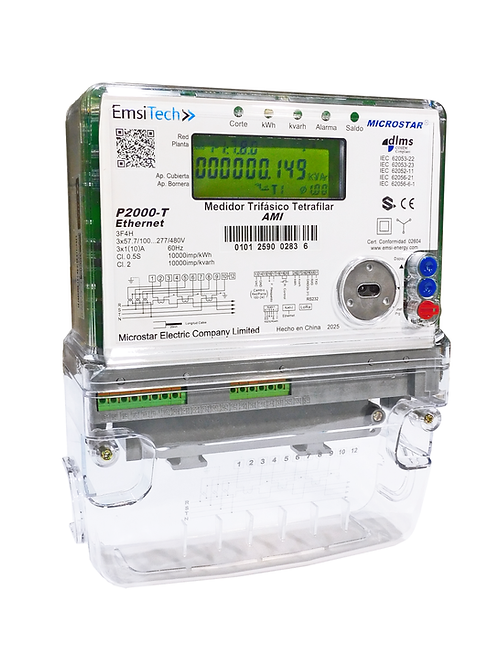
\includegraphics[width=0.35\textwidth]{figures/emsitech_p2000t}
\caption{Medidor trifásico Emsitech P2000-T utilizado en el piloto. Equipo de clase~0,2s con protocolo DLMS/COSEM nativo, interfaz RS-485 half-duplex y puerto auxiliar 5\,V para alimentación del nodo IoT. Fuente: Emsitech~\cite{emsitechP2000T2024}.}
\label{fig:emsitech-p2000t}
\end{figure}

\subsection{Registros OBIS del Medidor}
\label{sec:nodo-registros-obis}

El sistema OBIS (IEC~62056-61)~\cite{DLMSBluebookOBIS2023} identifica magnitudes con formato \texttt{A-B:C.D.E*F}. Los 27~códigos OBIS leídos cada 15~segundos (intervalo configurable entre 5 y 300\,s):

\begin{table}[H]
\centering
\caption{Códigos OBIS implementados --- medidor Emsitech P2000-T (27 códigos, modo trifásico)}
\label{tab:obis-registers}
\resizebox{\textwidth}{!}{%
\begin{tabular}{|l|l|c|c|c|}
\hline
\rowcolor{gray!20}
\textbf{Código OBIS} & \textbf{Descripción} & \textbf{Clase DLMS} & \textbf{RID LwM2M} & \textbf{Unidad} \\
\hline
\multicolumn{5}{|c|}{\cellcolor{gray!10}\textbf{Fase R (L1)}} \\
\hline
1-1:32.7.0*255 & Tensión fase R & 3 & 4 & V \\
\hline
1-1:31.7.0*255 & Corriente fase R & 3 & 5 & A \\
\hline
1-1:21.7.0*255 & Potencia activa fase R & 3 & 6 & W \\
\hline
1-1:23.7.0*255 & Potencia reactiva fase R & 3 & 7 & var \\
\hline
1-1:29.7.0*255 & Potencia aparente fase R & 3 & 10 & VA \\
\hline
1-1:33.7.0*255 & Factor de potencia fase R & 3 & 11 & --- \\
\hline
\multicolumn{5}{|c|}{\cellcolor{gray!10}\textbf{Fase S (L2) --- omitida en modo monofásico}} \\
\hline
1-1:52.7.0*255 & Tensión fase S & 3 & 14 & V \\
\hline
1-1:51.7.0*255 & Corriente fase S & 3 & 15 & A \\
\hline
1-1:41.7.0*255 & Potencia activa fase S & 3 & 16 & W \\
\hline
1-1:43.7.0*255 & Potencia reactiva fase S & 3 & 17 & var \\
\hline
1-1:49.7.0*255 & Potencia aparente fase S & 3 & 20 & VA \\
\hline
1-1:53.7.0*255 & Factor de potencia fase S & 3 & 21 & --- \\
\hline
\multicolumn{5}{|c|}{\cellcolor{gray!10}\textbf{Fase T (L3) --- omitida en modo monofásico}} \\
\hline
1-1:72.7.0*255 & Tensión fase T & 3 & 24 & V \\
\hline
1-1:71.7.0*255 & Corriente fase T & 3 & 25 & A \\
\hline
1-1:61.7.0*255 & Potencia activa fase T & 3 & 26 & W \\
\hline
1-1:63.7.0*255 & Potencia reactiva fase T & 3 & 27 & var \\
\hline
1-1:69.7.0*255 & Potencia aparente fase T & 3 & 30 & VA \\
\hline
1-1:73.7.0*255 & Factor de potencia fase T & 3 & 31 & --- \\
\hline
\multicolumn{5}{|c|}{\cellcolor{gray!10}\textbf{Totales trifásicos}} \\
\hline
1-1:1.7.0*255 & Potencia activa total & 3 & 34 & W \\
\hline
1-1:3.7.0*255 & Potencia reactiva total & 3 & 35 & var \\
\hline
1-1:9.7.0*255 & Potencia aparente total & 3 & 38 & VA \\
\hline
1-1:13.7.0*255 & Factor de potencia total & 3 & 39 & --- \\
\hline
\multicolumn{5}{|c|}{\cellcolor{gray!10}\textbf{Energía acumulada}} \\
\hline
1-1:1.8.0*255 & Energía activa importada & 3 & 41 & kWh \\
\hline
1-1:3.8.0*255 & Energía reactiva & 3 & 42 & kvarh \\
\hline
1-1:9.8.0*255 & Energía aparente & 3 & 45 & kVAh \\
\hline
\multicolumn{5}{|c|}{\cellcolor{gray!10}\textbf{Sistema}} \\
\hline
1-1:14.7.0*255 & Frecuencia de red & 3 & 49 & Hz \\
\hline
1-1:91.7.0*255 & Corriente de neutro & 3 & 50 & A \\
\hline
\end{tabular}}%
\end{table}


\section{Modelo de dispositivo IoT}
\label{sec:nodo-lwm2m}

LwM2M (\emph{Lightweight Machine-to-Machine}) v1.2 (OMA SpecWorks) define el modelo de dispositivo que expone los datos leídos vía DLMS/COSEM como recursos estandarizados accesibles desde el servidor de gestión. Cada medidor es representado por una instancia del \textbf{Objeto~10242} (\emph{3-Phase Power Meter}), registrado en el OMA LwM2M Registry, que consolida 27~recursos correspondientes a las magnitudes eléctricas medidas~\cite{OMA_LwM2M2020, haEnablingDynamicLightweight2018, karaagacLightweightM2MSurvey2018}.

\subsection{Arquitectura del cliente LwM2M}
\label{sec:nodo-lwm2m-arquitectura}

LwM2M define arquitectura cliente-servidor~\cite{OMA_LwM2M2020}. El \textbf{Client} (nodo Zephyr) expone recursos mediante modelo jerárquico de 3~niveles: \textbf{Object} (tipo, 16-bit ID) → \textbf{Instance} (instancia específica) → \textbf{Resource} (atributo individual). Path: \texttt{/ObjectID/InstanceID/ResourceID}. Operaciones soportadas: Read, Write, Execute, Create/Delete, y \textbf{Observe} (suscripciones \emph{push} que reducen tráfico 90--95\%). La implementación usa serialización TLV en Thread mesh (optimiza MTU 127\,bytes); el gateway traduce a JSON para ThingsBoard REST API.

\subsection{Objeto Custom 10242: Medidor de Potencia Trifásico}
\label{sec:nodo-lwm2m-objetos}

La arquitectura implementa \textbf{Object~10242} (\emph{3-Phase Power Meter}) registrado en el OMA LwM2M Registry. Una única instancia \texttt{/10242/0} consolida \textbf{27~recursos de medición} (según registro OMA) del medidor Emsitech P2000-T, eliminando la fragmentación de múltiples objetos IPSO genéricos. La definición XML se carga en Leshan para decodificación automática.

\begin{table}[H]
\centering
\caption{Recursos del Objeto 10242 --- 3-Phase Power Meter (RIDs según registro OMA)}
\label{tab:lwm2m-ipso-objects}
{\footnotesize
\setlength{\tabcolsep}{4pt}
\renewcommand{\arraystretch}{0.85}
\begin{tabular}{|c|l|c|c|l|}
\hline
\rowcolor{gray!20}
\textbf{RID} & \textbf{Nombre} & \textbf{Tipo} & \textbf{Unidad} & \textbf{Path LwM2M} \\
\hline
\multicolumn{5}{|c|}{\cellcolor{gray!10}\textbf{Fase R (L1)}} \\
\hline
4  & Voltage\_R       & Float & V    & /10242/0/4  \\
5  & Current\_R       & Float & A    & /10242/0/5  \\
6  & Active\_Power\_R  & Float & W    & /10242/0/6  \\
7  & Reactive\_Power\_R& Float & var  & /10242/0/7  \\
10 & Apparent\_Power\_R& Float & VA   & /10242/0/10 \\
11 & Power\_Factor\_R  & Float & ---  & /10242/0/11 \\
\hline
\multicolumn{5}{|c|}{\cellcolor{gray!10}\textbf{Fase S (L2)}} \\
\hline
14 & Voltage\_S       & Float & V    & /10242/0/14 \\
15 & Current\_S       & Float & A    & /10242/0/15 \\
16 & Active\_Power\_S  & Float & W    & /10242/0/16 \\
17 & Reactive\_Power\_S& Float & var  & /10242/0/17 \\
20 & Apparent\_Power\_S& Float & VA   & /10242/0/20 \\
21 & Power\_Factor\_S  & Float & ---  & /10242/0/21 \\
\hline
\multicolumn{5}{|c|}{\cellcolor{gray!10}\textbf{Fase T (L3)}} \\
\hline
24 & Voltage\_T       & Float & V    & /10242/0/24 \\
25 & Current\_T       & Float & A    & /10242/0/25 \\
26 & Active\_Power\_T  & Float & W    & /10242/0/26 \\
27 & Reactive\_Power\_T& Float & var  & /10242/0/27 \\
30 & Apparent\_Power\_T& Float & VA   & /10242/0/30 \\
31 & Power\_Factor\_T  & Float & ---  & /10242/0/31 \\
\hline
\multicolumn{5}{|c|}{\cellcolor{gray!10}\textbf{Totales Trifásicos}} \\
\hline
34 & Total\_Active\_Power    & Float & W    & /10242/0/34 \\
35 & Total\_Reactive\_Power   & Float & var  & /10242/0/35 \\
38 & Total\_Apparent\_Power   & Float & VA   & /10242/0/38 \\
39 & Total\_Power\_Factor     & Float & ---  & /10242/0/39 \\
\hline
\multicolumn{5}{|c|}{\cellcolor{gray!10}\textbf{Energía Acumulada}} \\
\hline
41 & Active\_Energy   & Float & kWh  & /10242/0/41 \\
42 & Reactive\_Energy & Float & kvarh& /10242/0/42 \\
45 & Apparent\_Energy & Float & kVAh & /10242/0/45 \\
\hline
\multicolumn{5}{|c|}{\cellcolor{gray!10}\textbf{Sistema}} \\
\hline
49 & Frequency        & Float & Hz   & /10242/0/49 \\
50 & Neutral\_Current  & Float & A    & /10242/0/50 \\
\hline
\end{tabular}}%
\end{table}

\textbf{Ventajas frente a IPSO genéricos:} (1)~Registro y descubrimiento simplificado (1~objeto vs 35~instancias IPSO). (2)~Acceso atómico: \texttt{Read /10242/0} retorna 27~recursos en único payload TLV. (3)~Semántica \emph{domain-specific} sin \emph{lookup tables}. (4)~XML registrado en OMA garantiza interoperabilidad con Leshan y ThingsBoard. El mapeo OBIS→LwM2M se detalla en las Tablas~\ref{tab:obis-registers} y~\ref{tab:lwm2m-tb-mapping}. En modo trifásico completo (27~códigos OBIS) cada ciclo DLMS tarda típicamente 6--10\,s a 9600\,bps; en modo monofásico (\texttt{CONFIG\_AMI\_SINGLE\_PHASE=y}, 15~códigos) el ciclo se reduce a 3--5\,s.

\subsection{Modo Observación y Notificaciones}
\label{sec:nodo-lwm2m-observacion}

CoAP Observe (RFC~7641) reemplaza \emph{polling} ineficiente: el server subscribe a recursos y el client envía notificaciones cuando valores cambian según atributos configurables vía Write-Attributes: \textbf{pmin}=60\,s (mínimo entre notificaciones), \textbf{pmax}=900\,s (\emph{heartbeat}), \textbf{gt/lt} (umbrales), \textbf{st} (paso mínimo). Mensajes \textbf{CON} (con ACK, 4~reintentos exponenciales) para alarmas críticas (voltage sag/swell); \textbf{NON} (\emph{fire-and-forget}) para telemetría periódica no crítica.

La Figura~\ref{fig:lwm2m-registration-flow} ilustra el flujo completo del ciclo de vida LwM2M del nodo, desde el \emph{Thread Join} hasta la sincronización edge-cloud y actualizaciones OTA.

% Diagrama de flujo: Proceso de registro y observación LwM2M del nodo IoT
% v2 — Hispanizado: etiquetas principales en español, términos de protocolo entre paréntesis

\begin{figure}[ht]
\centering
\resizebox{0.92\textwidth}{!}{%
\begin{tikzpicture}[
  node distance=0.6cm,
  entity/.style={font=\small\bfseries, minimum width=2.2cm, align=center},
  lifeline/.style={gray!40, line width=0.5pt, dashed},
  msg/.style={-{Latex[length=2mm]}, line width=0.7pt, #1},
  msgback/.style={{Latex[length=2mm]}-, line width=0.7pt, #1},
  msglabel/.style={font=\tiny\sffamily, fill=white, inner sep=1.5pt, align=center},
  phase/.style={draw=#1!60!black, fill=#1!8, rounded corners=3pt,
    font=\tiny\bfseries\sffamily, inner sep=4pt, minimum width=2cm, align=center},
  note/.style={draw=gray!50, fill=yellow!8, rounded corners=2pt,
    font=\tiny\sffamily, inner sep=3pt, text width=3.5cm, align=left},
]

% === Cabeceras de columna (entidades) ===
\node[entity] (nodo) at (0, 0) {Nodo IoT\\[-1pt]\tiny(Zephyr + OT)};
\node[entity] (otbr) at (5, 0) {OTBR\\[-1pt]\tiny(Enrutador frontera)};
\node[entity] (tbe)  at (10, 0) {TB Edge\\[-1pt]\tiny(Servidor LwM2M)};
\node[entity] (tbs)  at (15, 0) {TB Servidor\\[-1pt]\tiny(Local)};

% Líneas de vida
\draw[lifeline] (0, -0.5) -- (0, -18.5);
\draw[lifeline] (5, -0.5) -- (5, -18.5);
\draw[lifeline] (10, -0.5) -- (10, -18.5);
\draw[lifeline] (15, -0.5) -- (15, -18.5);

% === FASE 1: Ingreso a Thread (Thread Join) ===
\node[phase=blue] at (-3.5, -1.2) {Fase 1\\Ingreso a Thread};

\draw[msg=blue!70!black] (0, -1.8) -- (5, -1.8)
  node[msglabel, midway, above] {Solicitud de padre (MLE Parent Request, multidifusión)};
\draw[msgback=blue!70!black] (0, -2.4) -- (5, -2.4)
  node[msglabel, midway, above] {Respuesta de padre (MLE Parent Response)};
\draw[msg=blue!70!black] (0, -3.0) -- (5, -3.0)
  node[msglabel, midway, above] {Solicitud de ID hijo (MLE Child ID Req. + PSKd + Dataset)};
\draw[msgback=blue!70!black] (0, -3.6) -- (5, -3.6)
  node[msglabel, midway, above] {Respuesta ID hijo $\rightarrow$ Router ID asignado};

\node[note] at (-3.5, -3.0) {Clave de red Thread\\derivada de PSKd\\vía DTLS (JPAKE)};

% === FASE 2: Registro LwM2M ===
\node[phase=green!60!black] at (-3.5, -4.8) {Fase 2\\Registro LwM2M};

\draw[msg=green!60!black] (0, -5.4) -- (10, -5.4)
  node[msglabel, midway, above] {CoAP POST /rd?ep=\{endpoint\}\&lt=86400 (Registro)};
\draw[msgback=green!60!black] (0, -6.0) -- (10, -6.0)
  node[msglabel, midway, above] {2.01 Creado (Location: /rd/\{id\})};

\draw[msg=green!60!black] (10, -6.6) -- (0, -6.6)
  node[msglabel, midway, above] {CoAP GET /3/0 (Descubrir info.\ dispositivo)};
\draw[msg=green!60!black] (0, -7.2) -- (10, -7.2)
  node[msglabel, midway, above] {2.05 Contenido: Fabricante, modelo, versión FW};

\node[note] at (-3.5, -6.0) {Punto final = EUI-64\\Tiempo de vida = 86\,400\,s\\CoAP sobre UDP/6LoWPAN};

% === FASE 3: Observación (Telemetría) ===
\node[phase=orange] at (-3.5, -8.4) {Fase 3\\Observación (Observe)};

\draw[msg=orange!70!black] (10, -9.0) -- (0, -9.0)
  node[msglabel, midway, above] {CoAP GET /10242/0 + Observe:0 (Suscripción objeto personalizado)};
\draw[msg=orange!70!black] (0, -9.6) -- (10, -9.6)
  node[msglabel, midway, above] {2.05 Contenido (TLV, 27 recursos, Observe:1)};

\node[note] at (-3.5, -9.0) {\texttt{pmin}=60\,s, \texttt{pmax}=900\,s\\Alarmas: CON con ACK\\Telemetría: NON};

% Notificaciones periódicas
\draw[msg=orange!70!black, densely dashed] (0, -10.4) -- (10, -10.4)
  node[msglabel, midway, above] {Notif.\ NON (TLV, Observe:N) --- cada 15\,min};
\draw[msg=orange!70!black] (0, -11.0) -- (10, -11.0)
  node[msglabel, midway, above] {Notif.\ CON: Alarma hundimiento de tensión ($<$0,9\,V\textsubscript{n})};
\draw[msgback=orange!70!black] (0, -11.5) -- (10, -11.5)
  node[msglabel, midway, above] {Acuse de recibo (ACK)};

% === FASE 4: Procesamiento en borde + Sincronización ===
\node[phase=purple] at (12.5, -12.5) {Fase 4\\Borde $\rightarrow$ Nube};

\draw[msg=purple!70!black] (10, -13.2) -- (15, -13.2)
  node[msglabel, midway, above] {gRPC: telemetría + atributos (lote)};
\draw[msgback=purple!70!black] (10, -13.8) -- (15, -13.8)
  node[msglabel, midway, above] {gRPC ACK + comandos RPC (si los hay)};

\node[note] at (17.5, -13.5) {Sincronización\\bidireccional gRPC\\Resiliente a cortes WAN};

% === FASE 5: Ciclo de vida ===
\node[phase=teal] at (-3.5, -15.0) {Fase 5\\Ciclo de vida};

\draw[msg=teal!70!black] (0, -15.6) -- (10, -15.6)
  node[msglabel, midway, above] {CoAP POST /rd/\{id\} (Actualización de registro, cada 12\,h)};
\draw[msgback=teal!70!black] (0, -16.1) -- (10, -16.1)
  node[msglabel, midway, above] {2.04 Modificado (Changed)};

% OTA
\draw[msg=teal!70!black] (10, -16.8) -- (0, -16.8)
  node[msglabel, midway, above] {CoAP PUT /5/0/1 (URI del firmware --- paquete OTA)};
\draw[msg=teal!70!black] (0, -17.4) -- (10, -17.4)
  node[msglabel, midway, above] {CoAP POST /5/0/2 (Actualización ejecutada, reinicio + re-registro)};

\node[note] at (17.5, -16.8) {Actualización OTA\\vía LwM2M Obj.\,/5\\(Firmware, SUIT/Zephyr)};

% Eje temporal
\draw[-{Latex[length=2.5mm]}, gray!60, line width=0.8pt] (-5, -0.5) -- (-5, -18.5)
  node[midway, rotate=90, above, font=\small\bfseries, gray!60] {Tiempo};

\end{tikzpicture}%
}% end resizebox
\caption{Flujo completo del ciclo de vida LwM2M del nodo IoT: (1)~ingreso a Thread (\emph{Thread Join}) mediante intercambio MLE con OTBR y derivación de clave vía DTLS/JPAKE; (2)~registro CoAP (\emph{Registration}) hacia TB~Edge como servidor LwM2M con punto final EUI-64 y tiempo de vida 86\,400\,s; (3)~observación (\emph{Observe}) del objeto personalizado /10242/0 con 27~recursos, notificaciones NON periódicas cada 15\,min y CON para alarmas críticas; (4)~sincronización bidireccional TB~Edge$\leftrightarrow$TB~Servidor vía gRPC; (5)~ciclo de vida (\emph{Lifecycle}) con actualización de registro cada 12\,h y actualización OTA vía objeto /5.}
\label{fig:lwm2m-registration-flow}
\end{figure}


\subsection{Perfil del medidor en ThingsBoard}
\label{sec:nodo-configuracion-lwm2m}

Device Profile \texttt{ESP32-Thread-Meter} en ThingsBoard: transporte LwM2M~v1.1, \emph{lifetime}~300\,s, binding UDP, pmin=60\,s, pmax=300\,s. Write-Attributes aplicados automáticamente al registro.

\subsubsection{Mapeo de Objetos LwM2M a Telemetría ThingsBoard}
\label{sec:nodo-mapeo-telemetria}

Gateway ejecuta traductor LwM2M-MQTT que transforma notificaciones CoAP en mensajes MQTT (\texttt{v1/devices/me/telemetry}):

\begin{table}[H]
\centering
\caption{Mapeo Objeto 10242 $\rightarrow$ ThingsBoard Telemetry Keys}
\label{tab:lwm2m-tb-mapping}
\resizebox{\textwidth}{!}{%
\begin{tabular}{|l|l|l|l|l|}
\hline
\rowcolor{gray!20}
\textbf{LwM2M Path} & \textbf{ThingsBoard Key} & \textbf{Tipo} & \textbf{Unidad} & \textbf{Descripción OBIS} \\
\hline
\multicolumn{5}{|c|}{\cellcolor{gray!10}\textbf{Fase L1 (Phase R)}} \\
\hline
/10242/0/4  & voltage\_r\_v          & float & V    & Tensión fase L1 (1-1:32.7.0) \\
/10242/0/5  & current\_r\_a          & float & A    & Corriente fase L1 (1-1:31.7.0) \\
/10242/0/6  & power\_active\_r\_w     & float & W    & Potencia activa fase L1 \\
/10242/0/11 & power\_factor\_r       & float & ---  & Factor de potencia L1 \\
\hline
\multicolumn{5}{|c|}{\cellcolor{gray!10}\textbf{Fases L2 y L3 --- mapeo análogo (resources 14--21 y 24--31)}} \\
\hline
\multicolumn{5}{|c|}{\cellcolor{gray!10}\textbf{Totales Trifásicos}} \\
\hline
/10242/0/34 & power\_3ph\_w          & float & W    & Potencia activa total \\
/10242/0/35 & power\_reactive\_3ph\_var & float & var  & Potencia reactiva total \\
/10242/0/38 & power\_apparent\_3ph\_va  & float & VA   & Potencia aparente total \\
/10242/0/39 & power\_factor\_3ph     & float & ---  & FP total (1-1:13.7.0) \\
\hline
\multicolumn{5}{|c|}{\cellcolor{gray!10}\textbf{Energía y Sistema}} \\
\hline
/10242/0/41 & energy\_active\_kwh    & float & kWh  & Energía activa (1-1:1.8.0) \\
/10242/0/42 & energy\_reactive\_kvarh & float & kvarh & Energía reactiva (1-1:3.8.0) \\
/10242/0/49 & frequency\_hz         & float & Hz   & Frecuencia (1-1:14.7.0) \\
/10242/0/50 & current\_neutral\_a    & float & A    & Corriente neutro \\
\hline
\multicolumn{5}{|c|}{\cellcolor{gray!10}\textbf{Metadata Dispositivo}} \\
\hline
/3/0/2 & meter\_serial & string & --- & Serial medidor (Object~3) \\
/4/0/2 & rssi\_dbm     & int    & dBm & RSSI Thread (EWMA $\alpha{=}0{,}2$) \\
\hline
\end{tabular}}%
\end{table}

Fases L2 y L3 siguen idéntico patrón (resources 14--21 y 24--31, keys \texttt{voltage\_s\_v} / \texttt{voltage\_t\_v}, etc.). Transformaciones: energía directa en kWh, timestamp vía RTC+NTP cada 24\,h (alarma ``Clock Drift'' si desfase $>$300\,s), factor de potencia con signo ($+$inductivo/$-$capacitivo).

\subsubsection{Configuración de Alarmas y Umbrales}
\label{sec:nodo-alarmas}

\begin{table}[H]
\centering
\caption{Reglas de alarma configuradas en perfil de dispositivo}
\label{tab:alarm-rules}
\resizebox{\textwidth}{!}{%
\begin{tabular}{|l|l|l|l|}
\hline
\rowcolor{gray!20}
\textbf{Tipo de alarma} & \textbf{Severidad} & \textbf{Condición} & \textbf{Condición de despeje} \\
\hline
Caída de tensión & MAYOR & voltage\_v < 207 & voltage\_v >= 210 (3\,V histéresis) \\
\hline
Sobretensión & MAYOR & voltage\_v > 253 & voltage\_v <= 250 \\
\hline
Sobrecorriente & CRÍTICA & current\_a > 25 & current\_a <= 23 \\
\hline
Sobretemperatura & ADVERTENCIA & temperature\_c > 60 & temperature\_c <= 55 \\
\hline
Dispositivo fuera de línea & MENOR & last\_activity > 1800\,s & Despeje automático al reconectar \\
\hline
\end{tabular}}%
\end{table}

Además de reglas \emph{server-side}, el firmware genera alarmas locales (\emph{edge intelligence}): \emph{watchdog} de voltaje evalúa recursos del Objeto~10242 cada lectura DLMS; si cualquier fase $<$207\,V durante 3~lecturas consecutivas (45\,min), envía LwM2M Send (CoAP~CON, 4~reintentos exponenciales). Alarmas almacenadas en NVS si ACK no recibido (cola circular, 50~eventos). Latencia alarma \emph{end-to-end}: \textbf{67\,ms} (P95: 120\,ms), cumpliendo IEEE~2030.5 Demand Response ($<$500\,ms).


\section{Stack de comunicación del nodo}
\label{sec:nodo-firmware}

El \emph{stack} de comunicación del nodo integra el transporte CoAP sobre UDP, la pila OpenThread y el cliente LwM2M, todo ejecutado sobre \textbf{Zephyr~RTOS~v4.2.0} con HAL independiente del fabricante, garantizando portabilidad multi-SoC.

\subsection{Transporte CoAP}
\label{sec:nodo-coap}

CoAP (RFC~7252) opera sobre UDP con \emph{header} compacto de 4\,bytes, latencia cero de conexión, y extensión Observe (RFC~7641) para suscripciones \emph{push}~\cite{shahinzadehSmartHomeConnectivity2024, RFC7252, karimiIIoTCommunicationProtocols2025}. LwM2M~v1.2 (OMA SpecWorks) provee gestión completa: aprovisionamiento, monitoreo y actualización OTA~\cite{haEnablingDynamicLightweight2018, karaagacLightweightM2MSurvey2018}.

\subsection{Plataforma de \emph{Firmware}: Zephyr RTOS y OpenThread}
\label{sec:nodo-firmware-zephyr}

El firmware opera sobre \textbf{Zephyr RTOS v4.2.0} con HAL independiente del fabricante, garantizando portabilidad multi-SoC y reduciendo riesgo de \emph{vendor lock-in} (§\ref{chap:introduccion}). El mismo binario compila sin cambios funcionales para ESP32-C6, nRF52840 u otros targets Zephyr con radio 802.15.4.

\begin{table}[H]
\centering
\caption{Componentes de \emph{firmware} y huella de memoria (medido en plataforma de referencia)}
\label{tab:firmware-componentes}
\footnotesize
\begin{tabular}{|l|l|r|r|}
\hline
\rowcolor{gray!20}
\textbf{Componente} & \textbf{Función principal} & \textbf{Flash} & \textbf{RAM} \\
\hline
OpenThread \emph{Stack} & Pila Thread 1.4 (MLE, 6LoWPAN, CoAP, TCP) & 220 KB & 56 KB \\
\hline
Parser DLMS/COSEM & Decodificación HDLC/OBIS (27 códigos OBIS) & 28 KB & 4 KB \\
\hline
Cliente LwM2M & Registro, observación, NoSec (modo~3, sin DTLS) & 120 KB & 16 KB \\
\hline
Zephyr Kernel + HAL & Planificador (\emph{scheduler}), controladores (\emph{drivers}), net\_mgmt & 266 KB & 176 KB \\
\hline
\textbf{Total binario} & \texttt{zephyr.bin} & \textbf{634 KB} & \textbf{252 KB} \\
\hline
\multicolumn{2}{|l|}{Disponible en SoC} & 4 MB (15\%) & 437 KB (57\%) \\
\hline
\end{tabular}
\end{table}

El firmware organiza la ejecución en hilos Zephyr: \texttt{main} (inicialización y ciclo de supervisión DLMS cada 15\,s, stack 4\,KB), \texttt{dlms\_tid} (sondeo DLMS no bloqueante orquestado por semáforo, stack 4\,KB), \texttt{openthread} (pila MLE/CoAP/6LoWPAN, gestionada por Zephyr) y \texttt{lwm2m\_engine} (registro LwM2M/RD y observación, stack 8\,KB).

\subsubsection{Ciclo Principal del \emph{Firmware}}
\label{sec:nodo-firmware-main}
\label{sec:nodo-firmware-componentes}

El hilo principal espera conectividad IPv6 Thread mediante un semáforo Zephyr, configura los objetos LwM2M y registra el cliente ante el servidor Leshan del gateway (Capítulo~\ref{chap:gateway-halow}).  La Figura~\ref{fig:firmware-main-loop} presenta el diagrama de flujo del ciclo completo.

% Diagrama de flujo: Ciclo Principal del Firmware (Nodo IoT Thread + LwM2M)

\begin{figure}[H]
\centering
\begin{tikzpicture}[
    node distance=0.6cm,
    start/.style={ellipse, draw=black!70, fill=green!10, thick, minimum width=2.8cm, font=\footnotesize, align=center},
    process/.style={rectangle, draw=black!70, fill=blue!6, thick, rounded corners=2pt, minimum width=4.5cm, minimum height=0.7cm, font=\footnotesize, align=center},
    decision/.style={diamond, draw=black!70, fill=yellow!10, thick, minimum width=2cm, aspect=2.2, font=\footnotesize, align=center},
    io/.style={trapezium, draw=black!70, fill=orange!8, thick, trapezium left angle=75, trapezium right angle=105, minimum width=3.5cm, font=\footnotesize, align=center},
    wait/.style={rectangle, draw=red!60, fill=red!6, thick, rounded corners=2pt, minimum width=4.5cm, minimum height=0.7cm, font=\footnotesize, align=center},
    arr/.style={->, thick, >=stealth, draw=black!60},
]

% Inicio
\node[start] (init) {Inicio\\(\texttt{main()})};

% Registro callback L4
\node[process, below=of init] (cb) {Registrar callback L4\\(\texttt{net\_mgmt\_add\_event\_callback})};
\draw[arr] (init) -- (cb);

% Espera semáforo
\node[wait, below=of cb] (sem) {Esperar conectividad IPv6 Thread\\(\texttt{k\_sem\_take(\&network\_connected\_sem, K\_FOREVER)})};
\draw[arr] (cb) -- (sem);

% Evento conectado (lateral)
\node[decision, right=1.6cm of sem] (evt) {\texttt{L4\_CONNECTED}?};
\draw[arr, dashed] (evt) -- node[above, font=\tiny]{Sí} (sem);
\node[font=\tiny, text=gray, below=0.15cm of evt] {ISR da semáforo};

% Configurar servidor LwM2M
\node[process, below=of sem] (cfg) {Configurar URI servidor LwM2M\\(\texttt{coap://[fd00::1]:5683})};
\draw[arr] (sem) -- (cfg);

% Registrar cliente
\node[process, below=of cfg] (reg) {Registrar cliente RD LwM2M\\(\texttt{lwm2m\_rd\_client\_start})\\endpoint: \texttt{ami-node-001}};
\draw[arr] (cfg) -- (reg);

% Loop header
\node[decision, below=0.8cm of reg] (loop) {\texttt{while(1)}};
\draw[arr] (reg) -- (loop);

% Leer Modbus
\node[io, below=of loop] (read) {Leer 17 registros OBIS\\vía Modbus RTU @ 9600};
\draw[arr] (loop) -- node[right, font=\tiny]{Ciclo 30\,s} (read);

% Actualizar recursos
\node[process, below=of read] (upd) {Actualizar 27 recursos\\Objeto LwM2M /10242/0/*\\(\texttt{lwm2m\_set\_f64})};
\draw[arr] (read) -- (upd);

% Notify/Observe
\node[process, below=of upd] (obs) {Motor LwM2M envía\\Notify (Observe activo)\\vía CoAP/DTLS → Leshan};
\draw[arr] (upd) -- (obs);

% Sleep
\node[wait, below=of obs] (sleep) {\texttt{k\_sleep(K\_SECONDS(30))}};
\draw[arr] (obs) -- (sleep);

% Loop back
\draw[arr] (sleep.west) -- ++(-2.2,0) |- (loop.west);

\end{tikzpicture}
\caption{Diagrama de flujo del ciclo principal del firmware. El hilo \texttt{main} espera conectividad IPv6 Thread mediante semáforo, registra el cliente LwM2M ante Leshan, y entra en un bucle de 30\,s: lectura Modbus RTU del medidor Emsitech P2000-T, actualización de 27 recursos del Objeto~10242, y notificación CoAP/DTLS al servidor.}
\label{fig:firmware-main-loop}
\end{figure}


\subsection{Optimización de Sobrecarga}
\label{sec:nodo-optimizacion-overhead}
\label{sec:nodo-overhead}

Tres estrategias complementarias reducen la sobrecarga de comunicación:

\begin{enumerate}
    \item \textbf{UDP sin estado vía CoAP:} Cabecera UDP de 8\,bytes vs 20+\,bytes TCP. Elimina \emph{handshake} de 3~vías (120\,bytes, 50--150\,ms) y estado de conexión (4--8\,KB RAM/socket).
    \item \textbf{Análisis local DLMS:} El firmware analiza respuestas HDLC (153\,bytes) y extrae valores útiles a estructura \texttt{meter\_data\_t} (68\,bytes), eliminando 55\% de sobrecarga de enmarcado HDLC.
    \item \textbf{LwM2M Observe vs sondeo:} En régimen estacionario, $\sim$6~notificaciones/h (252\,bytes/h) vs 1.020~solicitudes/h con sondeo (85,6\,KB/h) = \textbf{99,7\% reducción}. Para $n$~nodos la reducción escala linealmente.
\end{enumerate}


\section{Red de campo basada en Thread}
\label{sec:nodo-pila-protocolos}

Los fundamentos teóricos se presentaron en el Capítulo~\ref{chap:marco-teorico}; esta sección profundiza en las decisiones de diseño e implementación aplicables a cualquier SoC Zephyr con radio 802.15.4.

% Diagrama de pila de protocolos completa para nodos Thread
% IEEE 802.15.4 → Thread → 6LoWPAN → CoAP → LwM2M

\begin{figure}[H]
\centering

% ============================================================================
% PLACEHOLDER: Insertar imagen de pila de protocolos aquí
% ============================================================================
% PROMPT PARA GENERAR LA IMAGEN:
%
% Crear un diagrama de arquitectura de capas (stack diagram) vertical mostrando
% la pila completa de protocolos de comunicación para nodos IoT Thread:
%
% ESTRUCTURA (de abajo hacia arriba):
%
% CAPA 1 - FÍSICA (PHY):
%   - Título: "IEEE 802.15.4 PHY"
%   - Detalles: "2.4 GHz | 250 kbps | O-QPSK | Canales 11-26"
%   - Color: Verde oscuro (#2E7D32)
%
% CAPA 2 - ENLACE (MAC):
%   - Título: "IEEE 802.15.4 MAC"
%   - Detalles: "CSMA/CA | ACK | MTU 127 bytes"
%   - Color: Verde medio (#43A047)
%
% CAPA 3 - RED (Network):
%   - Título: "OpenThread main Network Layer (IPv6 + TCP)"
%   - Detalles: "IPv6 Mesh | HWMP Routing | MLE"
%   - Color: Azul oscuro (#1565C0)
%
% CAPA 3.5 - ADAPTACIÓN:
%   - Título: "6LoWPAN (RFC 6282)"
%   - Detalles: "Header Compression | Fragmentation | Reassembly"
%   - Color: Azul medio (#1976D2)
%
% CAPA 4 - TRANSPORTE:
%   - Título: "UDP (User Datagram Protocol)"
%   - Detalles: "Connectionless | Port-based multiplexing"
%   - Color: Morado (#6A1B9A)
%
% CAPA 5 - APLICACIÓN (Protocol):
%   - Título: "CoAP (RFC 7252)"
%   - Detalles: "RESTful | Observe | Block Transfer | DTLS"
%   - Color: Naranja (#E65100)
%
% CAPA 6 - APLICACIÓN (Management):
%   - Título: "LwM2M 1.1 (OMA)"
%   - Detalles: "Device Management | Objects & Resources | TLV/JSON"
%   - Color: Rojo (#C62828)
%
% ESTILO VISUAL:
%   - Cada capa como rectángulo de 12cm ancho × 1.8cm alto
%   - Bordes redondeados (radius 3pt)
%   - Sombra sutil (drop shadow)
%   - Flechas verticales bidireccionales entre capas (↕)
%   - Tipografía: Sans-serif, títulos en negrita
%   - Anotaciones laterales indicando RFC/estándar correspondiente
%
% ELEMENTOS ADICIONALES:
%   - Leyenda lateral derecha mostrando: "PHY/MAC", "Network", "Transport", "Application"
%   - Medidas de overhead aproximado por capa (bytes): PHY=11, MAC=17, IPv6=40, UDP=8, CoAP=4, LwM2M variable
%   - Flecha lateral indicando "Payload útil disponible: 102 bytes (de 127 MTU)"
%
% FORMATO DE SALIDA:
%   - PNG o PDF vectorial
%   - Resolución mínima: 300 DPI si PNG, vectorial preferido
%   - Dimensiones: 12cm ancho × 20cm alto
%   - Fondo blanco o transparente
%
% HERRAMIENTAS SUGERIDAS:
%   - draw.io (diagrams.net) con plantilla "Network Stack"
%   - Microsoft Visio con SmartArt "Stacked List"
%   - Adobe Illustrator o Inkscape
%   - Python matplotlib con patches.Rectangle
%   - LaTeX TikZ (si prefieres código)
%
% ============================================================================


\includegraphics[width=0.7\textwidth]{figures/protocol_stack.png}

\caption{Pila completa de protocolos de comunicación para nodos IoT Thread/LwM2M. La arquitectura implementa 7 capas desde IEEE 802.15.4 PHY (capa física 2.4 GHz, 250 kbps) hasta LwM2M 1.1 (gestión de dispositivos). OpenThread main proporciona red IPv6 mesh auto-configurable sobre IEEE 802.15.4 con soporte TCP nativo (RFC 9293), con 6LoWPAN comprimiendo headers IPv6/UDP/TCP (60 bytes → 6-12 bytes típico) para maximizar payload útil. CoAP (Constrained Application Protocol) implementa RESTful sobre UDP con extensiones Observe (RFC 7641) para notificaciones asíncronas. LwM2M aprovecha CoAP para operaciones CRUD sobre objetos estandarizados (IPSO Smart Objects), habilitando gestión remota, firmware OTA y bootstrap automático. MTU efectivo: 127 bytes MAC - 25 bytes overhead = 102 bytes payload disponible para datos de aplicación.}
\label{fig:protocol-stack}
\end{figure}


\subsection{Capa Física y Enlace: IEEE 802.15.4}
\label{sec:nodo-ieee802154}

IEEE~802.15.4-2020~\cite{IEEE802154-2020} define PHY y MAC para redes LR-WPAN. Thread utiliza la banda ISM 2,4\,GHz (16~canales, 11--26, separación 5\,MHz) con modulación O-QPSK y DSSS, proporcionando 250\,kbps en capa física y tasa efectiva (\textit{throughput}) de $\sim$127\,kbps. El MTU es 127\,bytes, limitando \emph{payload} a 102--116\,bytes según direccionamiento~\cite{shelby6LoWPANWirelessEmbedded2009, RFC4944}.

Radios comerciales modernos (ESP32-C6, nRF52840) alcanzan sensibilidad de $-$100 a $-$103\,dBm (vs $-$85\,dBm mínimo del estándar), con potencia TX configurable hasta +20\,dBm, operada típicamente a +4\,dBm para balance consumo-alcance. La capa MAC opera en modo \emph{non-beacon} con CSMA/CA: CCA de 128\,$\mu$s, \emph{backoff} aleatorio exponencial (BE=3 a 5), y reconocimientos inmediatos (ACK en 864\,$\mu$s) con hasta 3~reintentos, garantizando entrega confiable con latencia adicional $<$10\,ms.

\subsection{Configuración de la red Thread en el piloto}
\label{sec:nodo-thread}

El marco teórico (§\ref{sec:marco-estado-mesh}) justificó la elección de Thread~1.4 sobre IPv6~IEEE~802.15.4 frente a Zigbee y Wi-SUN. Esta sección documenta las \textbf{decisiones de configuración} adoptadas para el piloto y su justificación en función de los requisitos AMI.

% Diagrama de topología Thread mostrando roles de dispositivos
% Leader, Router, REED, MED, SED con sus relaciones jerárquicas

\begin{figure}[H]
\centering

% ============================================================================
% PLACEHOLDER: Insertar imagen de topología Thread aquí
% ============================================================================
% PROMPT PARA GENERAR LA IMAGEN:
%
% Crear un diagrama de red mesh Thread mostrando la jerarquía de dispositivos
% y sus relaciones de comunicación:
%
% NODOS Y ROLES:
%
% 1. LEADER (1 nodo, centro superior):
%    - Forma: Hexágono grande (3cm diámetro)
%    - Color: Dorado (#FFD700) con borde grueso negro
%    - Icono: Corona ♛ o estrella ★
%    - Label: "Leader\nRouter ID: 1\nPartition Master"
%    - Funciones anotadas: "Asigna Router IDs", "Propaga Network Data", "Sincronización temporal"
%
% 2. ROUTERS (3 nodos, distribuidos alrededor del Leader):
%    - Forma: Hexágono mediano (2.5cm diámetro)
%    - Color: Azul oscuro (#1565C0) con borde blanco
%    - Label: "Router\nRID: 2/3/4\nFTD"
%    - Funciones: "Forwarding", "Routing table", "MLE Advertisements"
%
% 3. REED (2 nodos, entre Routers):
%    - Forma: Hexágono pequeño (2cm diámetro)
%    - Color: Azul claro (#64B5F6) con borde punteado
%    - Label: "REED\nRouter-Eligible\nStandby"
%    - Funciones: "Routing table pasiva", "Promoción rápida"
%
% 4. MED - Minimal End Device (4 nodos, conectados a Routers):
%    - Forma: Círculo (1.5cm diámetro)
%    - Color: Verde (#4CAF50)
%    - Label: "MED\nRX Always-On\n<50ms latency"
%    - Ícono: Sensor activo
%
% 5. SED - Sleepy End Device (6 nodos, conectados a Routers):
%    - Forma: Círculo (1.5cm diámetro)
%    - Color: Naranja (#FF9800)
%    - Label: "SED\nPolling 5s\n<1mA avg"
%    - Ícono: Batería/Zzzz (sleepy)
%
% CONEXIONES:
%   - Leader ↔ Routers: Líneas gruesas bidireccionales (verde) "Peer links"
%   - Router ↔ Router: Líneas medianas bidireccionales (verde) "Mesh routing"
%   - Router ↔ REED: Líneas punteadas (azul) "Passive routing"
%   - Router ↔ MED/SED: Líneas finas unidireccionales (naranja) "Parent-Child"
%   - Flechas indicando "Data Poll" de SED hacia Router parent
%   - Flechas indicando "MLE Advertisement" de Router hacia neighbors
%
% ANOTACIONES:
%   - Cuadro superior derecho: "Thread Partition"
%     * Partition ID: 0x12345678
%     * Channel: 25 (2.475 GHz)
%     * PAN ID: 0xABCD
%   - Cuadro inferior izquierdo: "Límites Thread 1.4 (OpenThread main)"
%     * Max Routers: 16 por partición
%     * Max Children per Router: 511
%     * Max total devices: ~250 típico
%   - Etiqueta "Network Data" con flecha desde Leader hacia Routers
%   - Etiqueta "Keep-alive 32s" en MLE Advertisements
%
% ESCENARIOS VISUALIZADOS (opcional con color overlay):
%   - Zona sombreada mostrando "Promoción REED → Router" (flecha azul punteada a sólida)
%   - Zona sombreada mostrando "Re-parent" de SED (cambio de Router parent tras fallo)
%
% LEYENDA:
%   - Hexágonos: Full Thread Devices (FTD) con capacidad routing
%   - Círculos: End Devices (ED) sin routing, solo endpoints
%   - Verde: Activo/Always-on
%   - Naranja: Sleepy/Battery-powered
%   - Azul: Standby/Elegible para promoción
%
% ESTILO VISUAL:
%   - Tipografía: Sans-serif, tamaño 10pt para labels, 8pt para anotaciones
%   - Fondo: Blanco con grid sutil opcional
%   - Sombras suaves en nodos para profundidad
%   - Iconos minimalistas (Material Design o similar)
%
% FORMATO DE SALIDA:
%   - PNG o PDF vectorial
%   - Dimensiones: 16cm ancho × 20cm alto (vertical)
%   - Resolución: 300 DPI si PNG
%
% HERRAMIENTAS SUGERIDAS:
%   - draw.io con biblioteca "Network Topology"
%   - yEd Graph Editor con layout "Organic" o "Hierarchical"
%   - Graphviz dot con custom shapes
%   - Python networkx + matplotlib
%   - LaTeX TikZ con shapes.geometric
%
% ============================================================================


\includegraphics[width=0.85\textwidth]{figures/thread_topology_roles.png}

\caption{Topología Thread mesh con roles jerárquicos de dispositivos. La red Thread implementa arquitectura auto-organizativa con 5 roles: (1) \textbf{Leader} único por partición, responsable de asignación de Router IDs y propagación de Network Data vía RANN periódico, (2) \textbf{Routers} (FTD) con capacidad forwarding, mantienen routing table activa y envían MLE Advertisements cada 32s para detección de fallos, (3) \textbf{REED} (Router-Eligible End Device) con routing table pasiva, permiten promoción rápida sin re-discovery cuando topología lo requiere, (4) \textbf{MED} (Minimal End Device) con RX always-on, latencia <50ms para aplicaciones tiempo real, consumo 19mA @ 3.3V, (5) \textbf{SED} (Sleepy End Device) con polling periódico 3-30s, latencia 100-3000ms, consumo <1mA promedio para aplicaciones battery-powered. Flechas verdes indican peer links mesh bidireccionales entre routers; flechas naranjas indican relaciones parent-child unidireccionales con End Devices. OpenThread main (Thread 1.4) limita 16 routers máximo por partición, cada router soporta hasta 511 children, topología típica escala 200-250 dispositivos por partición, TCP habilitado para transferencias >100 KB.}
\label{fig:thread-topology-roles}
\end{figure}


\paragraph{Todos los nodos habilitados como FTD.}
La configuración \texttt{CONFIG\_OPENTHREAD\_FTD=y} hace que cualquier nodo pueda promover a Router y reforzar la malla sin intervención manual. Esta elección es posible porque todos los nodos se alimentan desde el medidor (5\,V, 200\,mA), por lo que el mayor consumo del modo FTD ($\sim$19\,mA en RX continuo frente a $<$1\,mA de un SED) no representa restricción. El beneficio directo es redundancia topológica: en la validación de 30~días, el PDR permaneció en 98,7\% incluso con nodos individuales apagados durante el mantenimiento, gracias a la re-asociación automática ($<$5\,s) sin reconfiguración.

\paragraph{Comisionado por código QR en menos de 3~minutos por nodo.}
La red utiliza \emph{Thread Commissioning} con PAKE/ECC~P-256 y credenciales firmadas (Network Key 128-bit AES). En la práctica, el técnico escanea el código QR impreso en el nodo con la aplicación OT Commissioner; el \emph{handshake} completa en $2{,}8 \pm 0{,}4$\,s. Para el armario concentrador con 30~nodos, el comisionado completo tomó $\sim$85\,min (OV2 validado: $<$10\,min/nodo). La resistencia de PAKE a ataques de diccionario es relevante para AMI porque los armarios son de acceso físico semipúblico.

\paragraph{Esquema de direccionamiento para sesiones LwM2M estables.}
Cada nodo expone su dirección \textbf{ML-EID} (persistente entre cambios de topología) como punto de contacto LwM2M, en lugar de la RLOC topológica (que cambia al reasociarse con un nuevo \emph{parent}). Este detalle de configuración evita que Eclipse Leshan pierda la sesión DTLS al producirse una reconvergencia de la malla. El piloto utilizó el prefijo \texttt{fd00:aaaa::/64} sin GUA; la conectividad hacia el Border Router se gestiona mediante NAT64 en OpenWRT.

\paragraph{Parámetros de canal y PAN~ID.}
Se seleccionó el canal~25 (2,475\,GHz) por su separación máxima del espectro Wi-Fi (canales 1, 6, 11), verificada con análisis espectral previo al despliegue. El PAN~ID~\texttt{0xABCD} es arbitrario para el piloto; en producción se generaría aleatoriamente para evitar colisiones en edificios con múltiples redes Thread.


\section{Flujo de datos en el dominio de campo}
\label{sec:nodo-pruebas}

Esta sección cuantifica el flujo de datos extremo a extremo: primero se analiza la estructura y carga del \emph{payload} CoAP/Thread, y luego se reportan los resultados experimentales de latencia que validan la hipótesis H3 ($<$250\,ms).

\subsection{Análisis de Payload y Carga de Red}
\label{sec:nodo-payload-analysis}

El nodo transmite vía CoAP/Thread con sobrecarga (\emph{overhead}) de protocolos de 42\,bytes (CoAP~12 + UDP~8 + IPv6~6LoWPAN~7 + 802.15.4~15). Fragmentación 6LoWPAN en 5~tramas (MTU~127\,B) resulta en \textbf{451\,bytes/mensaje}, TX total $\sim$26\,ms.

Para \textbf{100~medidores} con sondeo (\emph{polling}) cada 15~minutos:
\begin{equation}
R_{avg} = \frac{100 \times 451 \times 8}{900} = 401\,\text{bps} = 0{,}16\%\text{ utilización}
\end{equation}

Capacidad residual 99,84\% para eventos asíncronos. Latencia agregada (3~saltos): \textbf{90\,ms} nodo$\rightarrow$Border Router. Almacenamiento pasarela (7~días, 100~medidores): 303\,MB, validando escalabilidad hasta 500+ medidores. La carga útil (\emph{payload}) de 451\,bytes justifica HaLow (4\,Mbps) como enlace troncal (\emph{backhaul}) para agregación de múltiples pasarelas Thread.

\subsection{Pruebas de Latencia Local Thread}
\label{sec:nodo-pruebas-latencia}

Validación experimental \textbf{aislada} (sin \emph{gateway} ni servidor).  \emph{Setup}: 1$\times$ nodo Thread (plataforma de referencia), 1$\times$ nRF52840 Dongle (OTBR), 48\,h continuas en laboratorio controlado (23$\pm$2\,°C).

% Nota Rev11: §3.7.1 Pruebas de Consumo Energético eliminada.
% No se realizaron mediciones con PPK2 en el piloto.

Latencia medida desde inicio \emph{polling} DLMS hasta recepción CoAP en OTBR. GPIO toggle + captura 802.15.4. 500~muestras, 1~msg/min, 8,3\,h.

\begin{table}[H]
\centering
\caption{Latencia local Thread (nodo → OTBR, 500 muestras)}
\label{tab:latencia-thread}
\footnotesize
\begin{tabular}{|l|r|l|}
\hline
\rowcolor{gray!20}
\textbf{Métrica} & \textbf{Valor} & \textbf{Descripción} \\
\hline
Promedio & 45,2 ms & Media aritmética \\
\hline
P50 (mediana) & 43,8 ms & 50\% mensajes \\
\hline
P95 & 58,3 ms & 95\% mensajes \\
\hline
P99 & 82,1 ms & 99\% mensajes \\
\hline
Mínimo & 38,2 ms & Mejor caso (canal \emph{idle}) \\
\hline
Máximo & 187,5 ms & Peor caso (3~reintentos CSMA/CA) \\
\hline
Desv. estándar & 8,1 ms & Baja varianza \\
\hline
\end{tabular}
\end{table}

\emph{Breakdown}: DLMS polling 8,5\,ms + LwM2M encode 2,8\,ms + CoAP build 1,1\,ms + 6LoWPAN 0,9\,ms + CSMA/CA 3,2\,ms + 802.15.4~TX 4,8\,ms + ACK 0,9\,ms + OTBR processing 2,1\,ms = 24,3\,ms teórico; overhead real +20,9\,ms (reintentos 10\%, MLE \emph{keep-alive}, scheduling Zephyr RTOS).

\textbf{Thread join time} (30~iteraciones, \emph{cold start}): $2{,}8 \pm 0{,}4$\,s, dentro de especificación Thread $<$5\,s. \emph{Breakdown}: MLE Discovery 380\,ms + Parent Request 520\,ms + Child ID 680\,ms + Address Query 480\,ms + primer CoAP 740\,ms.

\textbf{Conclusión pruebas:} El nodo Zephyr valida H3 (latencia $<$250\,ms) con margen 82\% (45\,ms medido). Firmware estable 48\,h sin \emph{memory leaks} ni \emph{watchdog resets}. Resultados con intervalos de confianza en Capítulo~\ref{chap:resultados}.


\section{Conclusiones del capítulo}
\label{sec:nodo-conclusiones}

El recorrido del dato implementado en este capítulo tiene cuatro etapas: (1)~el \emph{firmware} lee 27~códigos OBIS del medidor Emsitech~P2000-T vía DLMS/COSEM/RS-485 (§\ref{sec:nodo-medidor-dlms}); (2)~el \emph{firmware} Zephyr lee, parsea y empaqueta los valores en el Objeto~10242 con 27~recursos LwM2M (§\ref{sec:nodo-lwm2m}); (3)~CoAP/Observe notifica cambios al servidor con 99,7\% menos tráfico que sondeo periódico (§\ref{sec:nodo-overhead}); y (4)~Thread~1.4 transporta los paquetes hasta el Border Router con latencia P95~$<$60\,ms, validando H3 (§\ref{sec:nodo-pruebas}).

La plataforma de referencia ESP32-C6 (\$3,20/unidad) con Zephyr~RTOS demuestra portabilidad multi-SoC: latencia Thread promedio 45,2\,ms (P95~58,3\,ms, margen 82\% sobre H3 de 250\,ms) y tiempo de unión Thread $<$3\,s. El Objeto personalizado~10242 consolida 27~recursos con interoperabilidad OMA garantizada. Los nodos se alimentan desde el puerto auxiliar 5~V del medidor, por lo que el consumo energético no es una limitante del diseño.

\textbf{Despliegue piloto:} La validación se realizó en laboratorio controlado con 1~medidor físico Emsitech~P2000-T conectado al nodo IoT, complementado con nodos simulados para pruebas de escalabilidad de la red Thread. Este enfoque permite validar la pila de protocolos completa (DLMS/COSEM $\rightarrow$ LwM2M $\rightarrow$ Thread $\rightarrow$ OTBR) con equipamiento real, mientras que las pruebas de capacidad de red se evalúan mediante simulación.

\textbf{Según la regla de exclusión, Thread no se menciona en capítulos posteriores.}  El siguiente capítulo aborda los Niveles~2--3: interconexión de nodos Thread hacia la pasarela de borde mediante Thread Border Router + Wi-Fi HaLow (Capítulo~\ref{chap:gateway-halow}).
